\documentclass[conference]{IEEEtran}
\usepackage{graphicx,booktabs,amsmath,url}
\usepackage[hidelinks]{hyperref}
\usepackage{listings}
\lstset{basicstyle=\ttfamily\scriptsize,columns=fullflexible,keepspaces=true,frame=tb,framerule=0.4pt,
  keywordstyle=\bfseries,language=SQL,morekeywords={WITH,OVER,PARTITION,LAG,ROWS,UNBOUNDED,PRECEDING},aboveskip=3pt,belowskip=2pt}
\newcommand{\autos}{\textsc{auto\_suspend}}

\begin{document}
\title{Consolidate or Separate? Usually Neither:\\When Merging Cloud Data Warehouses Pays}

% AUTHOR LIST: confirm names, order and affiliations before Dec 1 (frozen after acceptance).
\author{\IEEEauthorblockN{Khadarvali Shaik}
\IEEEauthorblockA{[Affiliation -- non-academic]\\Richmond, VA, USA\\khadarvali.shaik@ieee.org}}

\maketitle

\begin{abstract}
Cloud data warehouses bill per second while running, with a minimum charge on each resume, so a fleet's bill depends on how
many warehouses it runs, which workloads share them, their sizes and when they suspend. Practitioners debate consolidating
warehouses to share idle time, yet no study measures when it pays. We replay two weeks of query history from Snowflake's
public fleet trace for 134 groups of warehouses that serve the same database, under a billing model that matches Snowflake's
actual running periods and running time to within 0.6\%, with size scaling measured on Snowflake. Searching layout,
size and auto-suspend jointly under a 1.2$\times$ latency bound, auto-suspend alone removes 24\% of the billed compute (60\% for the median group), assuming every warehouse runs
Snowflake's 600-second default, resizing almost never pays, and consolidation adds nothing for the median
group once suspend is tuned. Where it does pay---27 of 134 groups---it cuts the best tuned bill by 5--70\% (median 13\%),
and these few groups hold 98\% of the fleet's consolidation saving, 15\% of the tuned total; one 17-warehouse group holds
two thirds of it, and without that group consolidation adds 5.5\% of the tuned total. Contrary to the intuition that
merging helps lightly used warehouses share idle time, these are the groups whose warehouses run \emph{at the same time}:
merged, concurrent running time is billed once. A rule on the overlap of running periods, computed from query history alone,
identifies them with a leave-one-out balanced accuracy of 0.76. The findings hold across seven sensitivity settings. We release the replay tool and a one-query SQL check for overlap as open source.
\end{abstract}

\section{Introduction}
Most organisations do not run one Snowflake warehouse but dozens, created team by team and workload by workload. Each one
is billed for every second it runs and keeps running for a while after its last query~\cite{sf-warehouses,sf-create}, so
a team that issues a two-second dashboard query every few minutes pays mostly for idle time. Two remedies circulate among practitioners: lower the
auto-suspend timeout~\cite{sf-considerations}, and consolidate warehouses so that teams share one running warehouse instead of each
paying for its own tails. Vendor guidance discusses sizing~\cite{sf-considerations}; engine-side systems scale resources
automatically~\cite{rais24,scalesense26,costintel24}. None of these answers the question a platform team actually faces:
\emph{given our warehouses, should we merge some of them, and which?}

We answer it with a billing-exact replay of Snowflake's public fleet trace, Snowset~\cite{snowset}. Our contributions are
measurements, not a new optimizer:
\begin{itemize}
\item \textbf{Auto-suspend comes first.} Against the 600\,s default, tuning auto-suspend alone saves 24\% of billed compute
across 134 groups (median group 60\%); a joint search over layout, size and auto-suspend saves 35\%. Resizing almost never
pays under a latency bound.
\item \textbf{Consolidation rarely adds, but sometimes adds a lot.} Once auto-suspend is tuned, the median group gains 0\%
from merging. In 27 of 134 groups merging cuts the tuned bill by 5--70\%; one 17-warehouse group alone holds two thirds of
the fleet's consolidation saving, and without it consolidation adds 5.5\% of the tuned total.
\item \textbf{Overlap, not idleness, predicts when it pays.} We expected lightly used, idle-heavy warehouses to benefit. The
data say the opposite: merging pays when members' running periods overlap, because concurrent running time is billed once.
A rule on overlap alone reaches a leave-one-out balanced accuracy of 0.76.
\item \textbf{Validated on Snowflake.} The billing model matches the warehouse's own resume and suspend records; size scaling is
measured on Snowflake rather than assumed.
\end{itemize}
This paper asks only which warehouses should exist, not how the bill of a shared warehouse is divided among its users.

\section{Background}
\textbf{Billing.} A warehouse of size $s$ consumes credits at a rate proportional to $s$ (X-Small $=1$, doubling per size)
while running~\cite{sf-warehouses}. With per-second metering, a 60-second minimum per resume and an idle timeout $a$, the
billed time of a warehouse equals the measure of the union of $[\text{start}, \text{end} + a]$ over its queries when
$a \ge 60$; with shorter timeouts the resume minimum can add time. Merging two warehouses of equal size therefore saves the
time during which both would have run---their overlap---and the tails the merged warehouse no longer pays twice; it costs
queueing when the merged load exceeds the warehouse's concurrency. Figure~\ref{fig:mech} illustrates the two extremes.

\begin{figure}[t]
\centering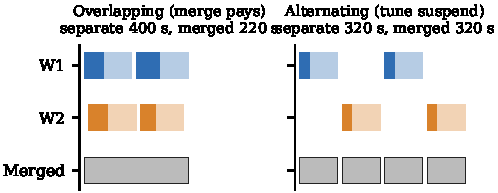
\includegraphics[width=\columnwidth]{figs/mechanism.pdf}
\caption{Why overlap decides. Solid: queries; light: 60\,s auto-suspend tails; grey: billed periods if merged. When two
warehouses run at the same time, merging bills the shared seconds once; when they take turns, merging saves nothing that a
short timeout has not already removed.}\label{fig:mech}
\end{figure}

\textbf{Related work.} Engine-side autoscaling chooses resources per query or workload inside one
service~\cite{rais24,scalesense26}; the cost-intelligence vision lets users state budgets instead of sizes~\cite{costintel24}.
Fleet traces such as Snowset~\cite{snowset} and Redset~\cite{redset} have been used to characterise workloads, not to evaluate
customer-side layout decisions. Server and virtual-machine consolidation packs workloads onto fewer hosts to save energy
under capacity constraints~\cite{beloglazov12}; in a per-second-billed warehouse the saving comes from time rather than
capacity---from seconds that several warehouses would each have been billed for---so the question of \emph{which} workloads
to merge has a different answer. Vendor guidance discusses auto-suspend and warehouse sizing~\cite{sf-considerations}; we found
no fleet-scale measurement of either remedy, or of consolidation.

\section{Design}
\textbf{Groups.} Snowset~\cite{snowset} records 69.2 million queries from 2,051 warehouses over 14 days in 2018, with
warehouse id, size and database id, but no customer id. As a same-customer proxy, a \emph{candidate group} is two or more
warehouses that each touch exactly one database, the same one, and keep one size throughout. There are 134 such groups
(388 warehouses; 89 pairs, 22 triples, 23 larger).

\textbf{Replay.} A query arrives at its observed execution start and runs for its observed execution time, rescaled to the
replayed size by $t' = t\,(s/s')^{\alpha(c)}$, where $c$ is a class by run time. Each warehouse has eight concurrent slots
(Snowflake's default) served first-come first-served; the first query after a suspend waits a one-second resume delay,
which is billed. Billing follows Section~II exactly.

\textbf{Options.} For each group we compare: (i) \emph{as-is}, every warehouse at its size with \autos{} 600\,s (also 60 and
300); (ii) \emph{resize only}, each warehouse at half, same or double size; (iii) \emph{tune auto-suspend only}, each warehouse
at 60, 300 or 600\,s; (iv) \emph{consolidate all} members into one warehouse, best feasible size and \autos{}; (v) the
\emph{joint search} over partitions of the group, sizes and \autos{} (exhaustive for up to four warehouses, greedy merging
beyond). Every option must keep each original warehouse's 95th-percentile latency within 1.2$\times$ its as-is value.

\section{Methodology}
\textbf{Pre-registration.} Group definition, options, latency bound, size-model protocol, rule search and sensitivity
variants were written down with timestamps before the corresponding runs. We disclose these deviations. (1)~The analysis keeps the
134 frozen groups although the runner also produced 21 groups after dropping size-changing members. (2)~The threshold for
``consolidation pays'' (5\%) was fixed after the main run, with features and rule search fixed before computing any feature.
(3)~An independent review found that the pre-registered analysis compared every option only on groups where \emph{all}
options were feasible, which silently dropped three groups (9, 17 and 2 warehouses) where consolidating everything breaks
the latency bound---including the group with the largest consolidation saving. We now compare as-is, single-knob and joint
options on all 134 groups and report consolidate-all on the 131 where it is feasible; on the old 131-group set,
auto-suspend saved 32\%, the joint search 37\%, and consolidation added 7.7\%. (4)~Our first rank correlation did not
average tied ranks; we report tie-corrected values. (5)~The SF100 size-scaling runs were added after the first block showed
every original statement finishing in under 3\,s at X-Small. (6)~Pre-registered secondary metrics not reported here: the
size model's leave-one-size-out error and the gap between greedy and exhaustive search.
Our stated expectation---that idle-heavy, lightly used groups would gain---was written before the features were computed and
turned out to be wrong.

\textbf{Size scaling on Snowflake.} On an X-Small/Small/Medium Generation 2 warehouse (query acceleration off) we ran 12
statements on a TPC-H-shaped schema and 6 TPC-H statements on Snowflake's SF100 sample data, in ABBA order
(XS, S, M, M, S, XS), three repetitions each with the first discarded, and fitted $\alpha$ per class from Snowflake's own
execution times (Table~\ref{tab:alpha}). Sub-second statements barely speed up; 10--60\,s statements scale almost linearly.
No statement exceeded 60\,s, so the longest class borrows the 10--60\,s value. The replay bills X-Small at one credit per
hour; the measured Generation~2 rate below is 1.35, which scales every bill equally and leaves percentages unchanged.

\begin{table}[t]
\caption{Measured size-scaling exponent $\alpha$ (execution time $\propto$ size$^{-\alpha}$).}\label{tab:alpha}
\centering\small
\begin{tabular}{lccc}
\toprule
Run time at XS & statements & $\alpha$ & note \\
\midrule
$<1$\,s & 10 & 0.34 & \\
1--10\,s & 6 & 0.75 & \\
10--60\,s & 2 & 0.96 & minimum sample \\
$>60$\,s & 0 & 0.96 & borrowed \\
\bottomrule
\end{tabular}
\end{table}

\textbf{How good is the size model?} Each of the 18 statements gives two observations (Small and Medium against
X-Small). Predicting each observation from its X-Small time and its class's $\alpha$ has a median error of 12.4\% (90th
percentile 44\%). Fitting $\alpha$ on one size and predicting the other gives a median error of 12.4\% (fit on Medium,
predict Small) and 24.8\% (fit on Small, predict Medium). Assuming no speed-up would err by a median 60\%, and linear
speed-up by 35\%. Individual sub-second statements scatter widely ($\alpha$ from $-0.26$ to $1.02$), which is why we vary
$\alpha$ by $\pm20\%$ in the sensitivity study (Table~\ref{tab:sens}).

\textbf{Billing validation on Snowflake.} On a dedicated X-Small warehouse we issued short probes separated by gaps around
the timeout and compared the model's running periods with the warehouse's own resume and suspend records. At \autos{} 300\,s the model
matched 4 of 4 periods and 99.8\% of running time; the warehouse suspended a median 300.5\,s after its last query. At 60\,s
it matched 7 of 7 periods and 99.4\% of running time, with a median tail of 60.1\,s. An administrator's session also ran
metadata statements on the warehouse during the 60\,s test; counting them as warehouse work would overstate running time by
8\%, because Snowflake runs such statements in its cloud-services layer without keeping the warehouse up. We ran this check on a warehouse of its own, independently of any other experiment. The metered rate
was 1.35 credits per running hour. Table~\ref{tab:f1} summarises the comparison.

\begin{table}[t]
\caption{Billing model vs.\ Snowflake's resume/suspend events (dedicated X-Small warehouse).}\label{tab:f1}
\centering\small
\begin{tabular}{lccc}
\toprule
Timeout & Periods (model/actual) & Time ratio & Median tail \\
\midrule
300\,s & 4 / 4 & 0.998 & 300.5\,s \\
60\,s & 7 / 7 & 0.994 & 60.1\,s \\
\bottomrule
\end{tabular}
\end{table}

\section{Results}
\textbf{Where the savings come from.} Figure~\ref{fig:savings} shows total billed compute saved relative to default
settings across the 134 groups (127,018 credits over two weeks at the replay's rate). Tuning auto-suspend saves 23.7\%; the
joint search saves 35.0\%. Resizing saves essentially nothing (under 0.1\%; it is strictly cheaper in three groups):
halving a warehouse slows sub-second queries by $2^{0.34} = 1.27\times$, past the 1.2$\times$ latency bound, and doubling
it does not speed them up enough to pay for the higher rate. This follows from the measured size model and the bound rather
than being a separate discovery: with $\alpha$ near 1, a larger warehouse costs the same per query; with $\alpha$ near
0.34, a smaller one is too slow. Consolidating every group into one warehouse (with its best
size and timeout) is infeasible in three groups and saves only 1.6\% in total on the other 131, although its per-group
median is 52.5\%: a few large groups cost far more merged. Per group, the median saving is 60\% for tuned auto-suspend and
61\% for the joint search. Figure~\ref{fig:cdf} shows the per-group view: the two curves nearly coincide.

\textbf{How much rests on one group?} Much of it. Without the 17-warehouse group described below, auto-suspend saves 25.3\%,
the joint search 29.4\%, and consolidation adds 5.5\% of the tuned total instead of 14.8\%, in 26 groups; without the two
largest, 2.8\%. The median-group result does not change. We read this as: consolidation is a large win for a few
organisations and a small one for the fleet.

\textbf{What if timeouts are already short?} Snowset records no suspend settings, so the as-is timeout is an assumption,
and it decides how much tuning can save. Against an as-is timeout of 600\,s (Snowflake's default) the joint search saves
35.0\% in total and a median 61\% per group; against 300\,s, 28.0\% and 46\%; against 60\,s, 14.8\% and 0\%. With 60\,s
already in place, tuning has nothing left to remove---in no group was a longer timeout cheaper---and the remaining 14.8\% is
consolidation alone, still concentrated in the same few groups. The consolidation result therefore does not depend on the
assumption; the auto-suspend result does.

\begin{figure}[t]
\centering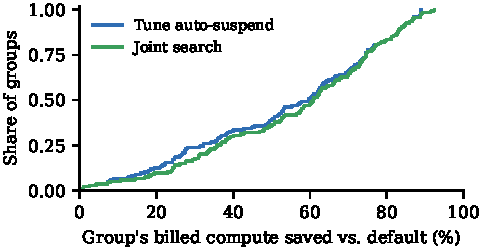
\includegraphics[width=\columnwidth]{figs/f3_cdf.pdf}
\caption{Per-group saving relative to default settings, 134 groups. The two curves nearly coincide: for most groups the
joint search adds little to tuning auto-suspend; the gap opens only in the few groups where consolidation pays.}\label{fig:cdf}
\end{figure}

\begin{figure}[t]
\centering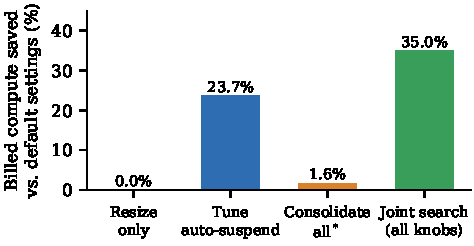
\includegraphics[width=\columnwidth]{figs/f3_savings.pdf}
\caption{Billed compute saved relative to default settings (\autos{} 600\,s), 134 groups, two weeks.
$^*$Consolidate-all: the 131 groups where it meets the latency bound.}\label{fig:savings}
\end{figure}

\textbf{What consolidation adds.} Relative to the better of resize-only and suspend-only, the joint search adds a median of
0\% (interquartile range 0--2.2\%) and 14.8\% of the total. It merges warehouses in 83 groups, but the merge cuts the
group's best single-knob bill by more than 5\% in only 27; where it does, by 5.1--70.3\% (median 12.7\%). The saving is
concentrated: one group accounts for 68.5\% of it and another for 17.5\%. Three examples show what the search does. The
largest is a 17-warehouse group (sizes 1 to 8; 3.7 million queries) in which every running period of every member overlaps
another member's: the search merges it into three warehouses (sizes 1, 4 and 8, all at 60\,s) and cuts the best single-knob
cost from 13,995 to 4,156 credits (70.3\%). In a six-warehouse group (sizes 4, 8, 8, 16, 32 and 64) it merges the four
smallest into one size-16 warehouse, keeps the 32 and 64 separate, and cuts 10,994 to 8,476 credits (22.9\%). In a
three-warehouse group (sizes 2, 1, 1; 632,030 queries; at least 98.9\% of each member's running periods overlap another's)
merging all three into one size-2 warehouse cuts 948 to 638 credits (32.7\%).

\textbf{Case study: the 17-warehouse group.} Figure~\ref{fig:case} shows six hours of this group's running periods at
60\,s. Over the 13.3 days of the trace, at least four of its warehouses were running at every moment, and 12.8 on average.
Run separately, the 17 warehouses accumulate 4,093 warehouse-hours of running time; billed at their sizes this is the
13,995 credits of the single-knob option (13,991 before the billed one-second resume delays). The three merged warehouses
each run for the whole trace, 960 warehouse-hours in all. Merging does not reduce how long compute
runs---the merged warehouses never suspend---but how many warehouses are billed for the same seconds. The merged
warehouses stay small (sizes 1, 4 and 8; no member was larger than 8) and still meet the latency bound. This is the case
our expectation got backwards: the members are busy, not idle---mean utilisation 42\%, against a median of 4\% across
groups---and they are worth merging precisely because they are running at the same time. Could they be one customer's multi-cluster
warehouse recorded as many? Not as recorded: Snowset gives each a separate warehouse id, and the members have four
different sizes (1, 2, 4 and 8), while the clusters of one multi-cluster warehouse share a size. The search's merged
warehouses also mix sizes. A multi-cluster warehouse is, however, a natural way to realise such a merge in practice, and we
note it as an alternative a platform team should weigh.

\begin{figure}[t]
\centering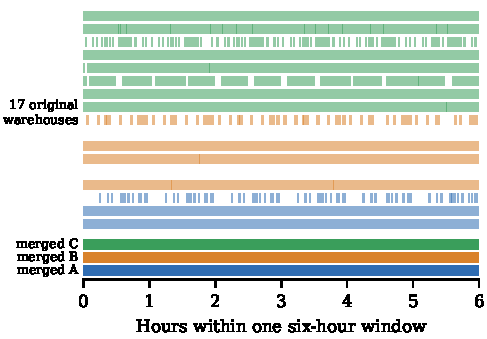
\includegraphics[width=\columnwidth]{figs/case17.pdf}
\caption{Case study: six hours of the 17-warehouse group at 60\,s auto-suspend. Upper rows: each original warehouse's
running periods, coloured by the merged warehouse the search assigns it to. Lower rows: the three merged warehouses, which
run continuously. Merging cuts the group's two-week bill from 13,995 to 4,156 credits.}\label{fig:case}
\end{figure}

\textbf{What the search chooses.} In every one of the 253 warehouses or merged warehouses in the joint plans, the search
picks the shortest timeout we allowed, 60\,s. It forms 91 merged warehouses, 69 of them pairs. Merging indiscriminately is
harmful: consolidating every group into one warehouse costs more than tuning auto-suspend alone in 68 of 131 groups, and more
than the default settings in 19.

\textbf{When it pays.} Among eleven group features computed from query history alone (Table~\ref{tab:feat}), the mean
overlap of members' running periods (at 60\,s auto-suspend) correlates most with the extra saving (Spearman $+0.51$). Group
size follows ($+0.32$); a wide spread of member sizes is negative ($-0.24$), since merging a small warehouse into a large one
bills its queries at the large rate. Idle share is weakly negative ($-0.20$), utilisation weakly positive ($+0.13$), and
resume frequency near zero. Figure~\ref{fig:overlap} shows the pattern. A depth-2 decision tree, evaluated by leave-one-out cross-validation, splits twice on the same feature and so reduces
to one rule---\emph{consolidate when mean overlap exceeds 0.55}---with balanced accuracy 0.76, precision 0.67 and recall
0.59 (baseline 0.50). A single threshold, also chosen inside each fold, lands lower (0.33) and reaches 0.71, but with
precision 0.41: overlap above one third is necessary rather than sufficient. The explanation is
the billing rule itself: two warehouses running in the same second are each billed for it, and merged they are billed once;
warehouses that take turns share only a tail, which tuning auto-suspend already removes.

\begin{table}[t]
\caption{Spearman correlation of group features with the extra saving from consolidation (134 groups; tie-corrected).
All features are computed from query history at 60\,s auto-suspend.}\label{tab:feat}
\centering\small
\begin{tabular}{lr@{\hspace{14pt}}lr}
\toprule
Feature & $\rho$ & Feature & $\rho$ \\
\midrule
Overlap, mean      & $+0.51$ & Idle share, min      & $-0.22$ \\
Overlap, min       & $+0.40$ & Idle share, mean     & $-0.20$ \\
Group size         & $+0.32$ & Resumes/day, mean    & $-0.06$ \\
Size spread        & $-0.24$ & Resumes/day, min     & $-0.07$ \\
Credits (60\,s)    & $+0.20$ & Utilisation, mean    & $+0.13$ \\
Utilisation, min   & $+0.12$ &                      &         \\
\bottomrule
\end{tabular}
\end{table}

\begin{figure}[t]
\centering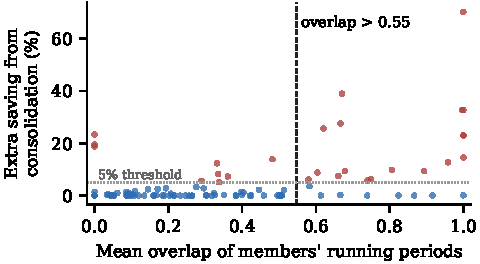
\includegraphics[width=\columnwidth]{figs/f4_overlap.pdf}
\caption{Extra saving from consolidation over the best single-knob option vs.\ the mean overlap of members' running periods
(134 groups). Red: groups where consolidation adds more than 5\%.}\label{fig:overlap}
\end{figure}

\textbf{Where the money is, and what the rule misses.} Table~\ref{tab:top} lists the eight groups with the largest
consolidation saving; together they hold 96\% of it. Five of the eight have a mean overlap of 1.0---every running period of
every member overlaps another member's---and all eight are above 0.55. Scored against the 27 groups where consolidation
pays, the overlap rule flags 18 correctly; those 18 hold 97.6\% of the fleet's consolidation saving. It misses 9, mostly
pairs of equal-size warehouses with low overlap (median 0.33) that gain a median 12\% but together account for only 0.6\%
of the saving. It wrongly flags 8, which gain a median of 0\%; their members differ in size by a median factor of four, so
merging moves small warehouses' queries onto a large warehouse's rate. A platform team can therefore read the rule as
``look here first'': it finds almost all of the money, and its false alarms tend to be groups of mixed sizes, which the
replay in the third step rejects. The
last column of Table~\ref{tab:top} also shows how much concurrency matters: with four slots instead of eight, the
six-warehouse group's gain falls from 22.9\% to 0.8\%, while the 17-warehouse group keeps 27.6\%.

\begin{table}[t]
\caption{The eight groups with the largest consolidation saving (two weeks). Best: cheaper of resize-only and
suspend-only; joint: joint search; share: of the fleet's total consolidation saving; 4 slots: extra saving with four
concurrency slots.}\label{tab:top}
\centering\scriptsize
\setlength{\tabcolsep}{2.6pt}
\begin{tabular}{rlrrrrcr}
\toprule
$k$ & sizes & best & joint & extra & share & overlap & 4 slots \\
\midrule
17 & 1--8           & 13{,}995 & 4{,}156 & 70.3\% & 68.5\% & 1.00 & 27.6\% \\
6  & 4,8,8,16,32,64 & 10{,}994 & 8{,}476 & 22.9\% & 17.5\% & 1.00 & 0.8\% \\
6  & 2,4,4,8,8,8    & 2{,}992  & 2{,}557 & 14.5\% & 3.0\%  & 1.00 & 14.5\% \\
3  & 1,1,2          & 948      & 638     & 32.7\% & 2.2\%  & 1.00 & 2.2\% \\
4  & 8,8,16,32      & 3{,}916  & 3{,}690 & 5.8\%  & 1.6\%  & 0.74 & 1.1\% \\
2  & 2,2            & 832      & 640     & 23.1\% & 1.3\%  & 1.00 & 23.1\% \\
2  & 4,16           & 4{,}819  & 4{,}644 & 3.6\%  & 1.2\%  & 0.58 & 3.6\% \\
3  & 4,4,8          & 488      & 363     & 25.7\% & 0.9\%  & 0.62 & 25.7\% \\
\bottomrule
\end{tabular}
\end{table}

\textbf{Sensitivity.} Table~\ref{tab:sens} repeats the full replay under seven one-at-a-time changes, each on all 134
groups. In every setting auto-suspend saves 22--24\%, the median extra from consolidation is at most 0.1\%, and overlap is
the strongest feature (Spearman $+0.42$ to $+0.59$). The fixed rule keeps a balanced accuracy of 0.71--0.87. Concurrency
matters most: with four slots instead of eight, merged warehouses queue, consolidation pays in only 16 groups and adds 5.3\%
of the total instead of 14.8\%.

\begin{table}[t]
\caption{Sensitivity: savings vs.\ defaults, groups where consolidation pays (${>}5\%$), and in-sample balanced accuracy of
the fixed overlap rule (mean overlap $>0.55$).}\label{tab:sens}
\centering\small
\setlength{\tabcolsep}{3.5pt}
\begin{tabular}{lcccc}
\toprule
Setting & suspend & joint & pays & rule acc. \\
\midrule
Main setting$^\dagger$ & 23.7\% & 35.0\% & 27 & 0.80 \\
Latency bound 1.1$\times$ & 23.6\% & 34.2\% & 31 & 0.75 \\
Latency bound 1.5$\times$ & 23.7\% & 35.5\% & 28 & 0.81 \\
4 concurrency slots & 23.0\% & 27.0\% & 16 & 0.71 \\
Resume delay 0\,s & 23.7\% & 35.0\% & 22 & 0.87 \\
Resume delay 5\,s & 22.3\% & 34.4\% & 36 & 0.73 \\
$\alpha \times 0.8$ & 23.7\% & 35.0\% & 27 & 0.80 \\
$\alpha \times 1.2^\ddagger$ & 23.7\% & 35.3\% & 29 & 0.77 \\
\bottomrule
\multicolumn{5}{l}{\footnotesize $^\dagger$ 1.2$\times$ bound, 8 slots, 1\,s resume delay, measured $\alpha$; 134 groups.}\\
\multicolumn{5}{l}{\footnotesize $^\ddagger$ Gives $\alpha > 1$ for queries over 10\,s; an optimistic bound.}\\
\end{tabular}
\end{table}

\section{A Playbook for Platform Teams}
The results suggest an order of operations. \emph{First}, set auto-suspend per warehouse from its own history; in our data
this captured two thirds of the available saving and needs no organisational change. \emph{Second}, for warehouses that serve the
same workload owner, compute the overlap of their running periods---the fraction of each warehouse's running periods that
intersect another member's. Figure~\ref{lst:overlap} computes it from query history with a 60\,s timeout using only
window functions; on the seven Snowset groups we re-ran, it reproduced the paper's overlap feature exactly, and it took
4\,s in DuckDB for the 17-warehouse group's 3.7 million queries. On Snowflake the input can come from
\texttt{QUERY\_HISTORY}, or the periods can be read directly from \texttt{WAREHOUSE\_EVENTS\_HISTORY}. \emph{Third}, consider merging only groups whose mean overlap exceeds about one half, and replay the
merge against a latency bound before acting: merged warehouses queue, and with low concurrency limits the benefit shrinks.
\emph{Do not} merge warehouses merely because they are idle most of the time; if they take turns, a shorter timeout already
removes their tails.

\begin{figure}[t]
\begin{lstlisting}
WITH tail AS (SELECT wh, s, e + 60 AS e FROM q),
reach AS (SELECT wh, s, e, MAX(e) OVER
    (PARTITION BY wh ORDER BY s, e ROWS BETWEEN
     UNBOUNDED PRECEDING AND CURRENT ROW) AS hi FROM tail),
gap AS (SELECT wh, s, e, CASE WHEN s > LAG(hi) OVER
    (PARTITION BY wh ORDER BY s, e) THEN 1 ELSE 0
    END AS brk FROM reach),
run_id AS (SELECT wh, s, e, SUM(brk) OVER (PARTITION
    BY wh ORDER BY s, e ROWS UNBOUNDED PRECEDING) AS r
    FROM gap),
period AS (SELECT wh, r, MIN(s) AS a, MAX(e) AS b
    FROM run_id GROUP BY wh, r),
shared AS (SELECT p.wh, p.r, MAX(CASE WHEN o.wh IS NULL
    THEN 0 ELSE 1 END) AS h FROM period p LEFT JOIN
    period o ON o.wh <> p.wh AND o.a <= p.b AND o.b >= p.a
    GROUP BY p.wh, p.r)
SELECT AVG(ov) AS mean_overlap FROM
  (SELECT wh, AVG(h) AS ov FROM shared GROUP BY wh) per_wh;
\end{lstlisting}
\caption{Mean overlap of a candidate group's running periods at 60\,s auto-suspend. Input: \texttt{q(wh, s, e)}, the
execution intervals of the group's queries. Consolidate when the result exceeds about 0.55.}\label{lst:overlap}
\end{figure}

\section{Implementation}
The replay tool reads per-warehouse query intervals, applies the size model and a first-come first-served multi-slot queue,
and bills with the exact per-second rules; the search enumerates set partitions for up to four warehouses (Bell(4) = 15) and
merges greedily beyond (13 of the 134 groups). The overlap query is released with it. The full Snowset replay of all 134 groups, including the joint search, ran in under five hours on a
laptop. A practical lesson from validation: statements that execute only in the cloud-services layer, such as grants and
\texttt{SHOW}, do not keep a warehouse running and must be excluded from the running-time model.

\section{Limitations}
Snowset is from 2018 and ran on older hardware; our size model rests on 18 statements, none longer than 60\,s, measured on
2026 Generation 2 warehouses, so scaling for longer queries is extrapolated. Snowset has no customer id or suspend events, so groups are a database-level proxy and
the as-is timeout is assumed (we report 60, 300 and 600\,s); the timeout grid stops at 60\,s. Concurrency is modelled as
eight first-come first-served slots, not Snowflake's resource-based limit. Arrivals are observed execution starts, so
original queueing is folded in; result-cache and local-cache effects are not modelled. The billing validation used one
X-Small warehouse with sequential probes; it did not exercise the 60-second minimum, concurrency, or merging. The
``pays'' threshold was set after the main run; at 3\% and 10\% the fixed rule's balanced accuracy is 0.79 and 0.77
(precision 0.73 and 0.38). The rule rests on 134 groups with 27 positives, and most of the saving sits in two groups.

\section{Future Work}
Validating the overlap rule on a current, customer-labelled fleet; modelling cache warmth when warehouses merge; and
extending the search to multi-cluster warehouses.

\section{Conclusion}
For a fleet of cloud warehouses, the first and largest saving is the auto-suspend timeout. Consolidation is not a general
remedy: it adds nothing for the median group. It pays---in one group by more than two thirds of the tuned bill---when
warehouses run at the same time, and query history is enough to find those groups.

\section*{Acknowledgment}
AI-generated content: Claude (Anthropic) was used to draft and edit the text, to write the analysis and replay code and the
SQL listing, and to produce the figures and tables in this paper. The author directed the study and ran the
experiments; every reported number was re-computed from the result files, and the author takes full responsibility for
the content.

\bibliographystyle{IEEEtran}
\bibliography{refs}
\end{document}
